\documentclass[11pt]{report}

\usepackage{report}
\usepackage[utf8]{inputenc} % allow utf-8 input
\usepackage[T1]{fontenc}    % use 8-bit T1 fonts
\usepackage[colorlinks=true, linkcolor=black, citecolor=blue, urlcolor=blue]{hyperref}       % hyperlinks
\usepackage{url}            % simple URL typesetting
\usepackage{booktabs}       % professional-quality tables
\usepackage{amsfonts}       % blackboard math symbols
\usepackage{nicefrac}       % compact symbols for 1/2, etc.
\usepackage{microtype}      % microtypography
\usepackage{graphicx}
\usepackage{doi}
\usepackage{tikz}
\usepackage{amsmath}
\usepackage{chemformula}
\usepackage{listings}
\usepackage{xcolor}
\usepackage{mwe}
\usepackage{siunitx}
\usepackage{appendix}
\usepackage[capitalise]{cleveref}
\creflabelformat{equation}{#2\textup{#1}#3}
\usepackage{amsthm}



\makeatletter
  \renewcommand*\tagform@[1]{\maketag@@@{Eq.~\ignorespaces #1\unskip\@@italiccorr}}
\makeatother


\definecolor{codegreen}{rgb}{0,0.6,0}
\definecolor{codegray}{rgb}{0.5,0.5,0.5}
\definecolor{codepurple}{rgb}{0.58,0,0.82}
\definecolor{backcolour}{rgb}{0.95,0.95,0.92}

\newcommand{\hly}[1]{\colorbox{yellow}{\parbox{\textwidth}{#1}}}
\newcommand\todo[1]{\textcolor{red}{#1}}


\lstdefinestyle{mystyle}{
    backgroundcolor=\color{backcolour},   
    commentstyle=\color{codegreen},
    keywordstyle=\color{magenta},
    numberstyle=\tiny\color{codegray},
    stringstyle=\color{codepurple},
    basicstyle=\ttfamily\footnotesize,
    breakatwhitespace=false,         
    breaklines=true,                 
    captionpos=b,                    
    keepspaces=true,                 
    numbers=left,                    
    numbersep=5pt,                  
    showspaces=false,                
    showstringspaces=false,
    showtabs=false,                  
    tabsize=2
}

\lstset{style=mystyle}

%% ========================
%% REMOVE BEFORE SUBMISSION
 \usepackage[angle=0, fontsize=0.05\paperwidth, vpos=0.027\paperheight, color=red]{draftwatermark}
%% ========================

%\setcitestyle{aysep={,}}
\renewcommand{\headeright}{M.Sc. Thesis}
\renewcommand{\shorttitle}{Simulating RFKO Slow Extraction}

\setlength{\parindent}{20pt}

\begin{document}
%%%%%%%%%%%%%%%%%%%%%%%%%%%%%%%%%%%%%%%%%
% University Assignment Title Page 
% LaTeX Template
% Version 1.0 (27/12/12)
%
% This template has been downloaded from:
% http://www.LaTeXTemplates.com
%
% Original author:
% WikiBooks (http://en.wikibooks.org/wiki/LaTeX/Title_Creation)
%
% License:
% CC BY-NC-SA 3.0 (http://creativecommons.org/licenses/by-nc-sa/3.0/)
% 
% Instructions for using this template:
% This title page is capable of being compiled as is. This is not useful for 
% including it in another document. To do this, you have two options: 
%
% 1) Copy/paste everything between \begin{document} and \end{document} 
% starting at \begin{titlepage} and paste this into another LaTeX file where you 
% want your title page.
% OR
% 2) Remove everything outside the \begin{titlepage} and \end{titlepage} and 
% move this file to the same directory as the LaTeX file you wish to add it to. 
% Then add \input{./title_page_1.tex} to your LaTeX file where you want your
% title page.
%
%%%%%%%%%%%%%%%%%%%%%%%%%%%%%%%%%%%%%%%%%
%\title{Title page with logo}
%----------------------------------------------------------------------------------------
%	PACKAGES AND OTHER DOCUMENT CONFIGURATIONS
%----------------------------------------------------------------------------------------
\begin{titlepage}

\newcommand{\HRule}{\rule{\linewidth}{0.5mm}} % Defines a new command for the horizontal lines, change thickness here
\center % Center everything on the page
 
%----------------------------------------------------------------------------------------
%	HEADING SECTIONS
%----------------------------------------------------------------------------------------

\textsc{\LARGE Royal Holloway University of London}\\[1.5cm] % Name of your university/college
\textsc{\Large M.Sc Thesis}\\[0.5cm] % Major heading such as course name
\textsc{\large Student ID: 100920158}\\[0.5cm] % Minor heading such as course title

%----------------------------------------------------------------------------------------
%	TITLE SECTION
%----------------------------------------------------------------------------------------

\HRule \\[0.4cm]
\begin{spacing}{2}
{ \huge \bfseries Comparative Analysis of Simulations and Experimental Outcomes: Slow Extraction Driven by RF Transverse Excitation at the CERN Proton Synchrotron}\\[0.4cm] % Title of your document
\end{spacing}
\HRule \\[0.4cm]

 
%----------------------------------------------------------------------------------------
%	AUTHOR SECTION
%----------------------------------------------------------------------------------------

\begin{minipage}{0.4\textwidth}
\begin{flushleft} \large
\emph{Author:}\\
Thomas \textsc{Bass} % Your name
\end{flushleft}
\end{minipage}
~
\begin{minipage}{0.4\textwidth}
\begin{flushright} \large
\emph{Supervisor:} \\
Professor Stephen \textsc{Gibson} % Supervisor's Name
\end{flushright}
\end{minipage}\\[2cm]

% If you don't want a supervisor, uncomment the two lines below and remove the section above
%\Large \emph{Author:}\\
%John \textsc{Smith}\\[3cm] % Your name

%----------------------------------------------------------------------------------------
%	DATE SECTION
%----------------------------------------------------------------------------------------

{\large \today}\\[2cm] % Date, change the \today to a set date if you want to be precise

%----------------------------------------------------------------------------------------
%	LOGO SECTION
%----------------------------------------------------------------------------------------


\includegraphics[width=0.25\linewidth]{Royal_Holloway_coat_of_arms.png}\\[1cm] % Include a department/university logo - this will require the graphicx package
 
%----------------------------------------------------------------------------------------

\vfill % Fill the rest of the page with whitespace

\end{titlepage}



\newpage
\tableofcontents
\thispagestyle{empty}

\newpage
\thispagestyle{empty}
\begin{abstract}
	\par{Resonant slow extraction is a beam extraction method which provides a continuous spill over a longer duration than can be achieved with fast single-turn or non-resonant multi-turn extraction. By using transverse excitation to drive the circulating particles onto the resonance, a beam can be delivered to fixed target experiments which require long-duration spills.}
\newline
	\par{In order to accurately and efficiently simulate the extraction process over a wide range of timescales, new modelling tools and computing platforms must be explored. By utilising optimised computational hardware - such as General Purpose Graphics Processing Units (GPGPUs), and next-generation simulation software (such as Xsuite), computation times for simulations can be reduced by several orders of magnitude.}
\newline
	\par{This thesis presents recent developments of resonant slow extraction modelling and benchmarking with a comparison to measurements made at CERN’s Proton Synchrotron (PS), with a particular focus on understanding the dynamics of transverse RF excitation and effect on spill quality.}


\end{abstract}

\newpage
%\setcounter{page}{1}
\chapter{Introduction}


The CERN Proton Synchrotron (PS), alongside providing intermediary acceleration for hadron and ion beams for the Super Proton Synchrotron (SPS) and eventually the Large Hadron Collider (LHC), provides beams for the many fixed target experiments located at the East Area (EA) experimental facility. This facility, as illustrated in \autoref{fig:eadiagram}, consists of the proton (IRRAD) and mixed-field (CHARM) irradiation facilities, via a dedicated \qty{24}{GeV/c} beamline, in addition to a multi-target beamline providing three secondary beams.

Ongoing experiments in these facilities such as the CHARM High-energy Ions for Micro Electronics Reliability Assurance (CHIMERA)~\cite{Fraser:feasibility} use high-Z ions (Pb) to simulate the harsh radiation environment of cosmic rays which satellites experience. Using low-intensity (\qty{<e6}{ions/spill}), high-energy (\qty{>100}{\MeV / u}) beams, customers such as the European Space Agency can assess the reliability of new materials in these environments. \autoref{fig:p_pb_injection} illustrates the two injection chains of the PS, either with Lead Ions sourced from the Linear Accelerator 3 (Linac3) and Low Energy Ion Ring (LEIR) chain, or Protons from the Linac4 and the Proton Synchrotron Booster (PSB).

\begin{figure}\label{fig:eadiagram}

\tikzset{every picture/.style={line width=0.75pt}} %set default line width to 0.75pt        
\begin{tikzpicture}[x=0.75pt,y=0.75pt,yscale=-1,xscale=1]
%uncomment if require: \path (0,300); %set diagram left start at 0, and has height of 300
%Shape: Arc [id:dp13623924019589717] 
\draw  [draw opacity=0][line width=3]  (23.16,157.13) .. controls (40.51,146.27) and (61.02,140) .. (83,140) .. controls (145.41,140) and (196,190.59) .. (196,253) .. controls (196,257.08) and (195.78,261.12) .. (195.36,265.09) -- (83,253) -- cycle ; \draw  [line width=3]  (23.16,157.13) .. controls (40.51,146.27) and (61.02,140) .. (83,140) .. controls (145.41,140) and (196,190.59) .. (196,253) .. controls (196,257.08) and (195.78,261.12) .. (195.36,265.09) ;  
%Straight Lines [id:da9881615579049192] 
\draw [line width=3]    (80,140) -- (540,140) ;
%Curve Lines [id:da41561885076946403] 
\draw [line width=3]    (160,140) .. controls (220.2,139.6) and (190.2,178.6) .. (260,180) ;
%Straight Lines [id:da9738553160260242] 
\draw [line width=3]    (260,170) -- (260,190) ;
%Curve Lines [id:da062105937338959416] 
\draw [line width=3]    (160,140) .. controls (220.2,139.6) and (190.2,98.6) .. (260,100) ;
%Curve Lines [id:da9621165186674936] 
\draw [line width=3]    (260,100) .. controls (320.2,99.6) and (320.2,68.6) .. (390,70) ;
%Curve Lines [id:da22957973507324092] 
\draw [line width=3]    (260,100) .. controls (320.2,99.6) and (470.2,98.6) .. (540,100) ;
%Curve Lines [id:da814674780127862] 
\draw [line width=3]    (390,70) .. controls (450.2,69.6) and (418.8,38.6) .. (540,40) ;
%Curve Lines [id:da1370169663287728] 
\draw [line width=3]    (390,70) .. controls (450.2,69.6) and (470.2,68.6) .. (540,70) ;
%Shape: Parallelogram [id:dp6647261304834908] 
\draw  [fill={rgb, 255:red, 80; green, 227; blue, 194 }  ,fill opacity=1 ] (477.7,30) -- (540,30) -- (532.3,50) -- (470,50) -- cycle ;
%Shape: Parallelogram [id:dp21515901263901416] 
\draw  [fill={rgb, 255:red, 80; green, 227; blue, 194 }  ,fill opacity=1 ] (367.7,129) -- (430,129) -- (422.3,149) -- (360,149) -- cycle ;
%Shape: Parallelogram [id:dp5134940082894275] 
\draw  [fill={rgb, 255:red, 80; green, 227; blue, 194 }  ,fill opacity=1 ] (457.7,129) -- (520,129) -- (512.3,149) -- (450,149) -- cycle ;
\draw  [fill={rgb, 255:red, 0; green, 0; blue, 0 }  ,fill opacity=1 ] (206,240) -- (196,260) -- (186,240) -- (196,250) -- cycle ;

% Text Node
\draw (141,121) node [anchor=north west][inner sep=0.75pt]   [align=left] {F61};
% Text Node
\draw (271,171) node [anchor=north west][inner sep=0.75pt]   [align=left] {F6D East Dump};
% Text Node
\draw (551,132) node [anchor=north west][inner sep=0.75pt]   [align=left] {T8 24 GeV/c};
% Text Node
\draw (241,82) node [anchor=north west][inner sep=0.75pt]   [align=left] {F62};
% Text Node
\draw (371,52) node [anchor=north west][inner sep=0.75pt]   [align=left] {F63};
% Text Node
\draw (551,32) node [anchor=north west][inner sep=0.75pt]   [align=left] {T11 3.5 GeV/c};
% Text Node
\draw (551,62) node [anchor=north west][inner sep=0.75pt]   [align=left] {T10 7 GeV/c};
% Text Node
\draw (551,92) node [anchor=north west][inner sep=0.75pt]   [align=left] {T9 15 GeV/c};
% Text Node
\draw (478.7,32) node [anchor=north west][inner sep=0.75pt]   [align=left] {CLOUD};
% Text Node
\draw (371.7,131) node [anchor=north west][inner sep=0.75pt]   [align=left] {IRRAD};
% Text Node
\draw (456.7,131) node [anchor=north west][inner sep=0.75pt]   [align=left] {CHARM};
% Text Node
\draw (114,246) node [anchor=north west][inner sep=0.75pt]   [align=left] {CERN PS};
\end{tikzpicture}
\caption{Layout diagram of the CERN East Area (EA) beamlines, their energies, and experiments.}

\end{figure}

\begin{figure}\label{fig:p_pb_injection}
\centering

\tikzset{every picture/.style={line width=0.75pt}} %set default line width to 0.75pt        

\begin{tikzpicture}[x=0.75pt,y=0.75pt,yscale=-1,xscale=1]
%uncomment if require: \path (0,300); %set diagram left start at 0, and has height of 300

%Straight Lines [id:da5948952889631192] 
\draw [line width=3]    (100,205) -- (164,204.6) ;
%Straight Lines [id:da30159595859877464] 
\draw [line width=3]    (100,50) -- (190,50) ;
%Curve Lines [id:da1754170813900049] 
\draw [line width=3]    (223,204.6) .. controls (262,204.6) and (261,163.6) .. (260,127.5) ;
%Shape: Parallelogram [id:dp44360400170472825] 
\draw  [fill={rgb, 255:red, 248; green, 200; blue, 220 }  ,fill opacity=1 ] (35.24,39.4) -- (110,39.4) -- (100.76,60) -- (26,60) -- cycle ;
%Shape: Circle [id:dp8675903510876994] 
\draw  [line width=3]  (157.5,82.5) .. controls (157.5,64.55) and (172.05,50) .. (190,50) .. controls (207.95,50) and (222.5,64.55) .. (222.5,82.5) .. controls (222.5,100.45) and (207.95,115) .. (190,115) .. controls (172.05,115) and (157.5,100.45) .. (157.5,82.5) -- cycle ;
%Straight Lines [id:da8930952466167899] 
\draw [line width=3]    (190,50) -- (337.5,50) ;
%Shape: Circle [id:dp4778308606413135] 
\draw  [line width=3]  (260,127.5) .. controls (260,84.7) and (294.7,50) .. (337.5,50) .. controls (380.3,50) and (415,84.7) .. (415,127.5) .. controls (415,170.3) and (380.3,205) .. (337.5,205) .. controls (294.7,205) and (260,170.3) .. (260,127.5) -- cycle ;
%Shape: Parallelogram [id:dp4706219846500248] 
\draw  [fill={rgb, 255:red, 200; green, 209; blue, 248 }  ,fill opacity=1 ] (35.24,194) -- (110,194) -- (100.76,214.6) -- (26,214.6) -- cycle ;
%Rounded Rect [id:dp7461155691700883] 
\draw  [line width=3]  (147,221.6) .. controls (147,212.21) and (154.61,204.6) .. (164,204.6) -- (223,204.6) .. controls (232.39,204.6) and (240,212.21) .. (240,221.6) -- (240,241.6) .. controls (240,250.99) and (232.39,258.6) .. (223,258.6) -- (164,258.6) .. controls (154.61,258.6) and (147,250.99) .. (147,241.6) -- cycle ;
%Straight Lines [id:da3035707453022254] 
\draw [line width=3]    (337.5,50) -- (437,50) ;
%Shape: Parallelogram [id:dp16470111074124638] 
\draw  [fill={rgb, 255:red, 80; green, 227; blue, 194 }  ,fill opacity=1 ] (417.7,41) -- (480,41) -- (472.3,61) -- (410,61) -- cycle ;
\draw  [fill={rgb, 255:red, 0; green, 0; blue, 0 }  ,fill opacity=1 ] (123,40) -- (143,50) -- (123,60) -- (133,50) -- cycle ;
\draw  [fill={rgb, 255:red, 0; green, 0; blue, 0 }  ,fill opacity=1 ] (123,195) -- (143,205) -- (123,215) -- (133,205) -- cycle ;
\draw  [fill={rgb, 255:red, 0; green, 0; blue, 0 }  ,fill opacity=1 ] (386,40) -- (406,50) -- (386,60) -- (396,50) -- cycle ;
\draw  [fill={rgb, 255:red, 0; green, 0; blue, 0 }  ,fill opacity=1 ] (411.14,175.85) -- (390,183.14) -- (396.85,161.86) -- (397,176) -- cycle ;
\draw  [fill={rgb, 255:red, 0; green, 0; blue, 0 }  ,fill opacity=1 ] (229.14,102.85) -- (208,110.14) -- (214.85,88.86) -- (215,103) -- cycle ;
\draw  [fill={rgb, 255:red, 0; green, 0; blue, 0 }  ,fill opacity=1 ] (250.14,249.85) -- (229,257.14) -- (235.85,235.86) -- (236,250) -- cycle ;

% Text Node
\draw (327,120) node [anchor=north west][inner sep=0.75pt]   [align=left] {PS};
% Text Node
\draw (41,62) node [anchor=north west][inner sep=0.75pt]   [align=left] {Protons};
% Text Node
\draw (424.7,43) node [anchor=north west][inner sep=0.75pt]   [align=left] {EAST};
% Text Node
\draw (41,42) node [anchor=north west][inner sep=0.75pt]   [align=left] {LINAC4};
% Text Node
\draw (174,74) node [anchor=north west][inner sep=0.75pt]   [align=left] {PSB};
% Text Node
\draw (41,196.6) node [anchor=north west][inner sep=0.75pt]   [align=left] {LINAC3};
% Text Node
\draw (39,175) node [anchor=north west][inner sep=0.75pt]   [align=left] {Lead Ions};
% Text Node
\draw (175,223) node [anchor=north west][inner sep=0.75pt]   [align=left] {LEIR};
% Text Node
\draw (180,122) node [anchor=north west][inner sep=0.75pt]   [align=left] {H+};
% Text Node
\draw (171,182) node [anchor=north west][inner sep=0.75pt]   [align=left] {Pb+54};
\end{tikzpicture}
\caption{Layout diagram of the two injection chains for the PS: either Protons (H+ ions) from Linac4, accelerated by the PSB; or Ions (Pb+54) from Linac 3, accelerated by the LEIR.}

\end{figure}

\section{Motivation}

The CHIMERA experiment, and other experiments located at the East Area and its SPS-sister-site North Area, are referred to as fixed-target experiments, to distinguish them from the collision experiments for which the LHC is most famous. The nature of these fixed-target experiments requires that a semi-continuous beam is delivered: if the entire energy of the PS was delivered to a material sample, for example, in an effectively instantaneous ``spill'' (a controlled removal of particles from the circular accelerator), any sensitive acquisition equipment would become saturated, and the fixed target itself likely destroyed. With the PS's revolution frequency typically around \qty{470}{kHz}, delivering particles over the period of one turn could, at most, provide a spill time on the order of \qty{2}{\micro\second}. This extraction method, known as ``fast'' extraction, is commonly used to transfer particles between successive accelerators, where the bunched time-structure of the beam must be preserved. To provide spills on the order of $\sim$\qty{100}{\ms} required for these experiments, a ``slow'' extraction system is employed.

\subsection{Performing Slow Extraction}
\begin{enumerate}
  \item \todo{Outlines the motivation behind performing Slow Extraction}
  \item \todo{Slow extraction is used where a spill has to be significantly longer than the revolution frequency}
  \item \todo{This has particular applications in medical and electronic reliability. Time structure is key}
  \item \todo{*Medical: its important to control dosage extremely precisely (why?)}
  \item \todo{Electronics reliability: CHIMERA STATUS \url{https://indico.cern.ch/event/1116677/contributions/4695314/attachments/2400040/4104314/CHIMERA\%20status\%20and\%20outlook.pdf}}
\end{enumerate}


In order to provide a long-duration spill, {\it slow extraction} must be used. Where fast extraction and injection methods utilise kicker magnets to move entire particle bunches between successive accelerators, slow extraction regimes rely on manipulating the beam to extract a small fraction of the available particles over a large number of turns. This regime produces the desired spill, but can be very sensitive to small changes of parameters. Accurately simulating the entire extraction process can often take tremendous processing power, as each of the $~10^{12}$ particles need to be tracked for many thousands of turns.

Therefore, to accurately simulate the spill produced by these extraction methods, one must first understand the fundamentals of accelerator beam dynamics, and grasp the technical challenges faced with simulation efforts. This thesis will first construct the required dynamic system of particle motion in a circular accelerator, and then introduce the theory behind slow extraction and the method used in this paper. Establishing a motivation for accurate and fast simulations slow extraction, various simulation methods will be presented, compared, and benchmarked with real-world data taken with the CERN PS.


\subsection{Simulating Slow Extraction}
\begin{enumerate}
  \item \todo{Outlines the motivation behind *simulating* SX}
  \item \todo{Long spills can be sensitive to small changes in conditions - understanding these is important}
  \item \todo{Many small/medical accelerators have high machine-on time and low machine demand, meaning they can test on accelerator rather than simulate}
  \item \todo{Smaller/medical accelerators tend to also be physically simpler}
  \item \todo{This is not afforded to CERN - many users competing for availability, highly complex system}
\end{enumerate}

\section{Challenges}
\begin{enumerate}
  \item \todo{Outlines the *challenges* with simulating SX}
  \item \todo{Simulating Fast extraction is well understood, as numerical models are easier (why? example?)}
  \item \todo{Simulating Fast extraction can typically happen over a very small number of turns}
  \item \todo{- Describe how Fast Extraction works optically}
\item \todo{- Provide an example: fast extraction at CERN SPS to LHC \url{https://cds.cern.ch/record/2674120/files/488.pdf}}
\end{enumerate}


\chapter{Theory}

\section{Single-Particle Transverse Beam Dynamics}

\subsection{Coordinate System}

The coordinate systems used to describe the dynamic motion of particles in a particle accelerator such as the PS relies on the periodic nature of a circular accelerator. Using a traditional Cartesian $x, y, z$ coordinate system would quickly introduce complications when describing circular trajectories, and so a local curvilinear coordinate system is used.

The basis vectors for this system, $(\hat x, \hat y, \hat s)$, constantly rotate in Cartesian space as the reference particle moves along the orbit of the accelerator. The longitudinal vector $\hat s$ is tangent to the particle's orbit, and the $\hat x$ direction is parallel to the radius of the accelerator. The absolute direction of $\hat y$ does not change, but makes one complete rotation in one closed orbit of the reference particle through the accelerator. This system is shown in Figure~\ref{fig:frenet-serret}, along with the radius of the circular trajectory $\rho$, and the angle from the origin $s=0$. 

\begin{figure}[!h]
\begin{center}
\tikzset{every picture/.style={line width=0.75pt}} %set default line width to 0.75pt        

\begin{tikzpicture}[x=0.75pt,y=0.75pt,yscale=-1,xscale=1]

%uncomment if require: \path (0,455); %set diagram left start at 0, and has height of 455

%Shape: Ellipse [id:dp0798878508534051] 
\draw   (142,162.5) .. controls (142,129.09) and (199.08,102) .. (269.5,102) .. controls (339.92,102) and (397,129.09) .. (397,162.5) .. controls (397,195.91) and (339.92,223) .. (269.5,223) .. controls (199.08,223) and (142,195.91) .. (142,162.5) -- cycle ;
%Straight Lines [id:da3917612889933506] 
\draw    (269.5,162.5) -- (269.5,57) ;
\draw [shift={(269.5,55)}, rotate = 90] [color={rgb, 255:red, 0; green, 0; blue, 0 }  ][line width=0.75]    (10.93,-3.29) .. controls (6.95,-1.4) and (3.31,-0.3) .. (0,0) .. controls (3.31,0.3) and (6.95,1.4) .. (10.93,3.29)   ;
%Straight Lines [id:da9587552919771436] 
\draw    (397,162.5) -- (269.5,162.5) ;
%Straight Lines [id:da15722891342539147] 
\draw    (269.5,162.5) -- (322.59,215.59) ;
\draw [shift={(324,217)}, rotate = 225] [color={rgb, 255:red, 0; green, 0; blue, 0 }  ][line width=0.75]    (10.93,-3.29) .. controls (6.95,-1.4) and (3.31,-0.3) .. (0,0) .. controls (3.31,0.3) and (6.95,1.4) .. (10.93,3.29)   ;
%Straight Lines [id:da7846346908558013] 
\draw    (324,217) -- (242.93,235.34) ;
\draw [shift={(240,236)}, rotate = 347.25] [fill={rgb, 255:red, 0; green, 0; blue, 0 }  ][line width=0.08]  [draw opacity=0] (10.72,-5.15) -- (0,0) -- (10.72,5.15) -- (7.12,0) -- cycle    ;
%Straight Lines [id:da569421074096844] 
\draw    (324,217) -- (324,141) ;
\draw [shift={(324,138)}, rotate = 90] [fill={rgb, 255:red, 0; green, 0; blue, 0 }  ][line width=0.08]  [draw opacity=0] (10.72,-5.15) -- (0,0) -- (10.72,5.15) -- (7.12,0) -- cycle    ;
%Straight Lines [id:da7806312488509295] 
\draw    (324,217) -- (345.88,238.88) ;
\draw [shift={(348,241)}, rotate = 225] [fill={rgb, 255:red, 0; green, 0; blue, 0 }  ][line width=0.08]  [draw opacity=0] (10.72,-5.15) -- (0,0) -- (10.72,5.15) -- (7.12,0) -- cycle    ;
%Curve Lines [id:da9180655893242637] 
\draw    (280,173) .. controls (284,177) and (291,162) .. (287,163) ;

% Text Node
\draw (406,153.4) node [anchor=north west][inner sep=0.75pt]    {$s=0$};
% Text Node
\draw (294,166.4) node [anchor=north west][inner sep=0.75pt]    {$\theta $};
% Text Node
\draw (271,177.4) node [anchor=north west][inner sep=0.75pt]    {$\rho $};
% Text Node
\draw (320,113.4) node [anchor=north west][inner sep=0.75pt]    {$\hat{y}$};
% Text Node
\draw (224,230.4) node [anchor=north west][inner sep=0.75pt]    {$\hat{s}$};
% Text Node
\draw (350,244.4) node [anchor=north west][inner sep=0.75pt]    {$\hat{x}$};


\end{tikzpicture}
\end{center}
\caption{The {\it Frenet-Serret} vectors used to define the coordinate system used in particle beam dynamics.}\label{fig:frenet-serret}
\end{figure}

This coordinate system is academically known as a {\it Frenet-Serret} type coordinate system, and can be rigorously defined by the unit vector {\it tangent} to the curve $\hat T$ (pointing in the direction of motion), the unit vector {\it normal} to the tangent and on the tangential plane $\hat N$, and the binormal unit vector $\hat B$, the cross product of $\hat T$ and $\hat N$. These unit vectors, forming an orthonormal basis spanning $\mathbb{R}^3$, and known collectively as the {\bf TNB} frame, are equal to the vectors $\hat x, \hat y, \hat s$ by:
\begin{equation}
\begin{pmatrix}\hat T\\\hat N\\\hat B \end{pmatrix}=\begin{pmatrix}\hat s\\-\hat x\\\hat y \end{pmatrix}
\end{equation}

The coordinate system $(\hat x, \hat y, \hat s)$ relies on the right-hand chirality (Figure~\ref{fig:rhr}) of the vector cross product for the $\hat x$ vector to point radially outwards from the centre of the machine, the $\hat y$ vector points upwards, and the $\hat s$ vector points in the direction of motion. The direction of $\hat x$ to point outwards from the centre of revolution is chosen as injection and extraction line apertures will therefore be located in the positive $\hat x$.

\begin{figure}[!h]
\begin{center}
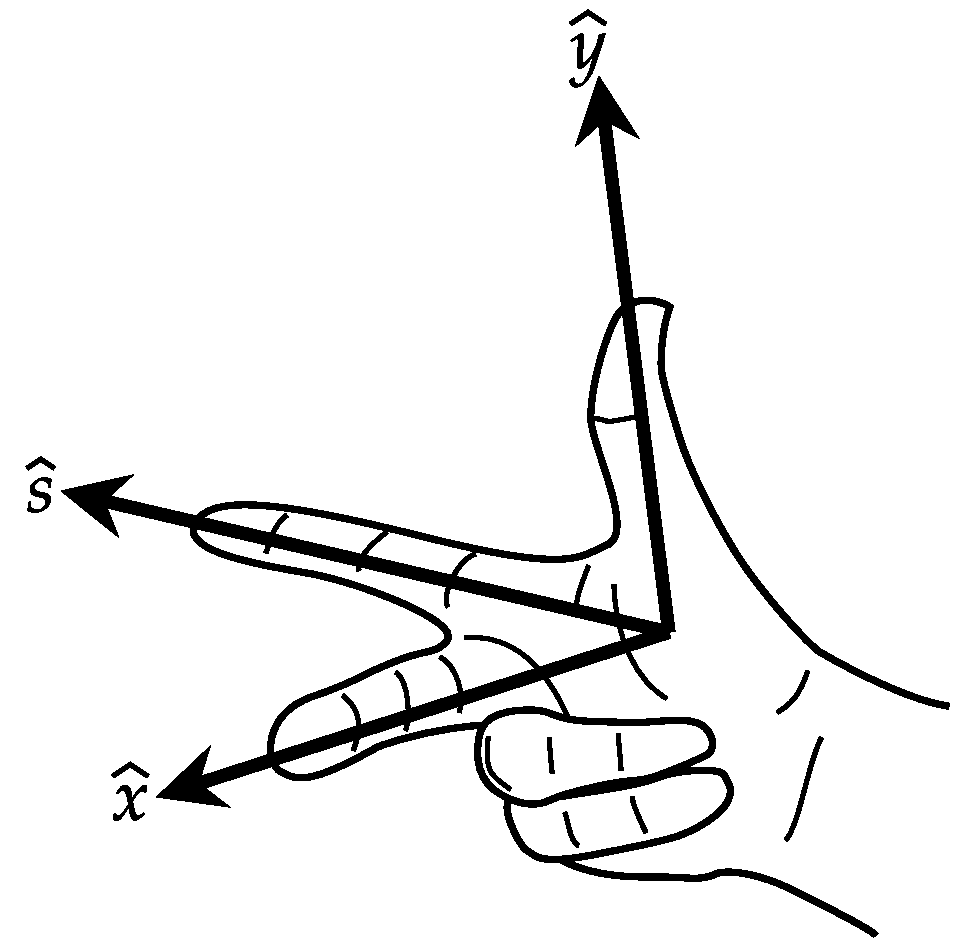
\includegraphics[scale=.25]{rhr.pdf}
\caption{The right-hand chirality rule defining the direction of $\hat s = \hat x \times \hat y$}
\label{fig:rhr}
\end{center}
\end{figure}

\subsection{Variable Space}
\begin{enumerate}
  \item \todo{6D space fully describes particles}
  \item \todo{4D space describes transverse motion - can be understood separately}
  \item \todo{Differences in variables between simulation software}
\end{enumerate}


\subsection{Ring Geometry}

\todo{Lorentz force balances centrifugal force - understanding of beam rigidity}
\begin{enumerate}
    \item \todo{Design orbit created by dipoles}
    \item \todo{Focussing created by quadrupoles}
    \item \todo{Non-Linear effects created by Sextupoles}
\end{enumerate}


All descriptions of particle accelerators are build upon the Lorentz force, describing the force $\vec F$ acting on a charged particle with charge $q$ as it moves through an electric field $\vec E$ and magnetic field $\vec B$ with velocity $\vec v$, given as
\begin{equation}
\vec F_{\text{lorentz}} = q\cdot(\vec E+ \vec v\times\vec B)\label{eq:lorentz}
\end{equation}
This equation can already show why magnetic fields are used in almost all areas of particle acceleration, and not electric fields; a particle with higher velocity $v$ will experience a greater force from a constant magnetic field $\vec B$, whereas the contribution from the electric field $\vec E$ will remain constant. Therefore, at velocities approaching the speed of light ($v \rightarrow c$), we can begin to neglect $\vec E$ for some derivations.

The other force experienced by a particle in an accelerator is the centripetal\footnote{while the coordinate system used allows for a reference frame whose orientation follows the orbit, this frame is not co-moving with the particles, but still fixed in the ``laboratory'' frame - otherwise, complex Lorentz transformations would be required.} force:
\begin{equation}
\vec F_{\text{centrif.}}=\frac{m_0v^2}{\rho}\label{eq:centrifugal}
\end{equation} where $m_0$ is the particle's rest mass, and $\rho$ is the radius of the particle's orbit inside the accelerator.

Equating equations \ref{eq:centrifugal} and \ref{eq:lorentz} yields
\begin{equation}
B\rho=\frac pq
\end{equation}
The quantity $B\rho$ is known as the {\t momentum rigidity} of a beam, and defines the bending angle of a particle for a given magnetic field. 

If the momentum $p=mv$ of the particle is measured in \unit[per-mode = symbol]{\GeV\per\clight\per amu}, and A and Ze are the atomic mass number and charge of the particle, the momentum rigidity can be expressed in Tesla-meters:

\begin{equation}
B\rho\ \left[\unit{\tesla\meter}\right]=\frac pq=\frac AZ\times3.33564\times q\ \left[\unit[per-mode=symbol]{\GeV\per\clight\per\atomicmassunit}\right]
\end{equation}

However, this formulation only describes a single magnetic field. In order to bend the particles along a circular trajectory, dipole magnets are used to create near-constant fields through which the particles travel. Again referring to Equation~\ref{eq:lorentz} (with the help of Figure~\ref{fig:rhr}), a magnetic field pointed vertically upwards (along the $\hat y$ vector) will cause a particle with motion along the $\hat s$ vector to experience a bending force along the $-\hat x$ direction.

The arrangements of these bending magnets - referred to as Main Units (MU) - will define the closed loop of one orbit in the accelerator - the {\it design orbit}.

If $\alpha$ is the bending angle of a single MU, then $\alpha$ can be related to the momentum rigidity by
\begin{equation}
\alpha=\frac{ds}\rho=\frac{B\ ds}{B\rho}
\end{equation}
Integrating this over all magnets in the ring, therefore, must be equal to one full revolution, $2\pi$
\begin{equation}
\frac{\int B\ ds}{B\rho}\equiv2\pi
\end{equation}

This result may seem obvious, but it is an important step in understanding why the transverse motion (i.e. that in the $\vec x$ and $\vec y$ directions) can be understood and analysed separately from that of the longitudinal ($\vec s$) motion. This result also provides one of the first key insights which is not obvious at first - that ``circular'' accelerators are in fact n-sided polygons, with bending magnets at each vertex, and a {\it drift} (accelerator sections without any significant electromagnetic field) or other non-bending multipole magnet at each side: in the case of the LHC, 1,232 dipole magnets are used to keep the beam on it's circular path; in the PS - 100. 

While the arrangement of these magnets - referred to as the {\it lattice} - is intended to create the design orbit, alignment errors, instabilities, and non-linearities create the actual closed-loop orbit of the machine - the {\it reference orbit}.

\hly{\textcolor{red}{is it more correct to say that the quadrupoles are {\it part} of the MUs? or are the MUs just the dipoles and\\ separate from focussing?}}


\section{Multi-particle Transverse Beam Dynamics}


While the configuration of the MU bending magnets, in addition to drifts and other higher-order magnets (discussed shortly), defines the design orbit of a single ideal particle, an accelerator beam is comprised of a great number of particles grouped together into one {\it bunch} - on the order of $10^{12}$ for the PS. These particles naturally have small variations in their initial position, angle, and momenta. The evolution of these changes in position and angle, with respect to the reference orbit, is understood through separating the longitudinal motion from motion in the transverse plane.

In the transverse dynamics of an accelerated beam, the {\it betatron function} refers to one of the three functions ($\alpha$, $\beta$, and $\gamma$), which, along with betatron phase $\mu$, can provide an emittance-independent representation of the properties of the beam. These functions are known as the {\it Twiss} or {\it Courant-Snyder} parameters of a transverse dynamics system. In a periodic (circular) accelerator, the linear equation for transverse equation takes the form of a Hill differential equation:
\begin{equation}
\frac{d^2x}{ds^2}-K(s)\cdot x(s)=0
\end{equation} where $x$ is the transverse displacement as a function of longitudinal position $s$, and $K$ is the focussing coefficient. Following Floquet's theorem \cite{Rossbach:247501}, general solution to this equation takes the form of the harmonic oscillator 
\begin{equation}
x(s) =\sqrt{\varepsilon}\sqrt{\beta(s)}\cos(\varphi(s)-\varphi_0)
\end{equation} where $\varphi$ is the phase of oscillation, $\varphi_0$ is the initial condition, $\varepsilon$ is an invariant property of the ensemble of particles (emittance), and $\beta(s)$ is an amplitude function. Taking the derivative with respect to $s$ gives an equation for the angle of the trajectory:
\begin{equation}
x'(s)=\sqrt{\varepsilon}\sqrt{\beta(s)}\left(\frac12\beta'(s)\cos(\varphi(s)-\varphi_0)+\sin(\varphi(s))\right)
\end{equation}

From these solutions, we can obtain an equation to describe phase advance of the oscillation:
\begin{equation}
\varphi(s)=\int^s_0\frac{ds}{\beta(s)}
\end{equation}

Basic analysis of this equation shows that at locations with large $\beta$ amplitude (and thus a large transverse displacement), phase advance $\varphi$ is small, and vice versa. The number of transverse oscillations per turn, the {\it tune} of the machine, is therefore defined as
\begin{equation}
Q=\frac1{2\pi}\oint\frac{ds}{\beta(s)}
\end{equation}

Momentum compaction factor

Gamma factor

Transverse tune = betatron tune

Long tune = synchrotron tune

Normalised emittance is constant under adiabatic damping

\subsection{Multi-particle Transverse Dynamics}\label{sec:theory-transverse}
\begin{enumerate}
    \item \todo{1. Relativistic beta, gamma}
    \item \todo{Twiss, momentum compaction, emittance, constant emittance (e.g. adiabatic damping)}
    \item \todo{How tune emerges, Adiabatic tune changes}
\end{enumerate}

\subsection{Multi-particle Longitudinal Dynamics}
\begin{enumerate}
    \item \todo{Tomography and Tomoscope}
    \item \todo{Longitudinal Emittance}
\end{enumerate}


\section{Slow Extraction}

\begin{enumerate}
  \item \todo{Machine resonance at third order, leading to a derivation of the Kobayashi Hamiltonian and Steinbach diagram}
  \item \todo{COSE (chromatic)}
  \item \todo{Q-sweep}
  \item \todo{Betatron}
  \item \todo{\textbf{RFKO} INTRODUCE RFKO FORMALLY HERE}
  \item \textcolor{teal}{Mathematical description of the four regimes}
  \item \textcolor{teal}{Perform these four extraction regimes}
  \item \textcolor{teal}{Demonstrate why RFKO is of interest}
\end{enumerate}

An analysis of RFKO begins with understanding transverse resonance effects in an accelerator. Particles which start with non-zero initial conditions are subject to transverse oscillations as they progress longitudinally - this is known as {\it betatron} oscillation. A consequence of this oscillation is that particles at different transverse positions will experience different bending (dipole) and focussing (quadrupole) forces \textcolor{red}{due to fringe fields or errors in magnets.} This leads to an energy spread in the machine. A {\it multi-energetic} beam will therefore have a spread of momenta, referred to as $dp-d-p_0$, the relative momentum deviation. A particle with $dp>0$ will require an orbit with large radius, and vica-versa.

It is easily understood that magnets of order $n$ create instabilities at the $n^{{th}}$ order tune. We start with an understanding of how slight variations in initial conditions of a beam causes dispersion. With reference to an {\it equilibrium orbit} (an orbit which passes through the exact centre of all dipoles and quadrupoles), a range of initial position distributions will cause particles at different spatial coordinates to experience different forces from magnets. This leads to a transverse oscillation around the equilibrium orbit which we understand as {\it betatron oscillation}, with the tune $Q$ of a machine being the number of betatron oscillations completed per revolution.

This ``energy spread'' necessarily leads to a momentum spread, which we understand as either purely relative or normalised deviation from the equilibrium momentum $p_0$:
\begin{equation}
 dp=p-p_0;\ \frac{dp}{p_0}=\frac{p-p_0}{p}
\end{equation}
We already understand that the particle's trajectories are defined by a differential equation\textcolor{red}{CITE}, which takes the form of
\begin{equation}
\frac{d^2x}{ds^2}+K(s)x=\frac 1\rho\frac{\Delta p}{p_0}
\end{equation} where $K(s)$ the normalised quadrupole strength;
\begin{equation}
K(s)=-\left(k(s)-\frac 1{\rho(s)^2}\right)
\end{equation}
 $\frac 1\rho$ is the dipole strength (the reciprocal of the equilibrium radius). The solution to this equation is the sum of the general and particular solutions, the first of which.

\chapter{Simulation and Benchmarking}
\section{Simulation Methodology}
\todo{\textbf{Focussed on original contribution}}
\begin{enumerate}
    \item \todo{What tools are available? MAD-X, MapTrack, Henontrack, Xsuite}
    \item \todo{How do they compare?} \textcolor{teal}{Accuracy studies between basic simulations}
    \item \todo{How extraction can be implemented in them: MAD-X limitation of sub-turn frequencies; Xtrack Exciter element}
    \item \todo{How extraction compares} \textcolor{teal}{spill accuracy studies between simulations and machine data}
    \item \todo{How performance compares} \textcolor{teal}{performance studies between SX simulations on CPU and GPGPU}
\end{enumerate}

\chapter{Conclusion}

\chapter{Acknowledgements}

\chapter{Bibliography}

\nocite{*}
\bibliographystyle{IEEEtran} % We choose the "plain" reference style
\bibliography{refs} % Entries are in the refs.bib file

\begin{appendices}

\chapter{Derivations}

\section{Relating longitudinal variables}

In order to relate the dispersive and chromatic functions produced by \verb|MAD-X| to those calculated by \verb|Xtrack|, we must multiply \verb|MAD-X|'s results by the relativistic Lorentz factor $\beta=v/c$. This is because \verb|MAD-X| uses the relative momentum error $\delta_p$ as a longitudinal variable, defined as
\begin{equation}
\delta_p=\frac{p-p_0}{p_0}
\end{equation}, where $p$ is the momentum of the particle, and $p_0$ the momentum of the {\it reference} (or {\it design}) particle, whereas \verb|Xtrack| uses the relative energy error

\chapter{Code Snippets}

\chapter{Data and Plots}

\end{appendices}

\end{document}
